\section{Il metodo \textit{Clone()}}
Il metodo \textit{clone()} restituisce un nuovo oggetto il cui stato iniziale è una copia dell’oggetto su cui viene invocato.

Se si vuole che sia possibile copiare gli oggetti di una classe, la classe deve implementare l’interfaccia \textit{Cloneable}.
Il metodo clone() che viene ereditato dalla classe Object controlla prima di tutto che la classe dell’oggetto implementi l’interfaccia Cloneable e in caso contrario lancia l’eccezione \textit{CloneNotSupportedException}, altrimenti crea un nuovo oggetto e lo inizializza con una copia degli attributi dell’oggetto originale; al termine restituisce un riferimento al nuovo oggetto.

Per garantire che il metodo Clone() non sia invocato accidentalmente, il metodo è dichiarato protected. Essendo dichiarato protected, per essere reso disponibile per l'invocazione nelle nostre classi bisognerà sottoporlo a override cambiandone il modificatore a public, come nel seguente esempio:

\begin{lstlisting}
public class Quadrato implements Cloneable {
...
   public Object clone() {
      try {
         Object ogg = super.clone();
         return ogg;    
      }    
      catch(CloneNotSupportedException e ){
         return null;
      }
  }    
       
}
\end{lstlisting}
È importante notare che la copia che viene fatta dal metodo \textit{Clone()} della classe Object, si limita a copiare i valori delle variabili d'istanza dell'oggetto (si tratta di shalllow copy o copia superficiale).Quindi se le variabili d'istanza sono reference ad altri oggetti, allora verranno copiati i loro indirizzi, e non il contenuto del reference creandosi cosi una condivisione di memoria.
\begin{figure}[H]
\centering
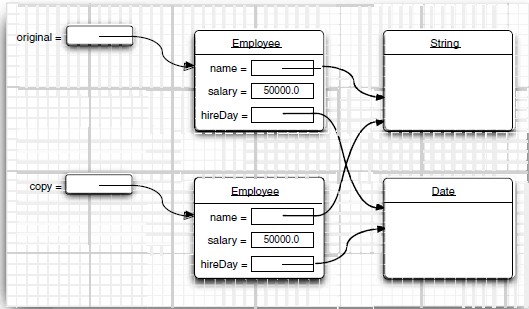
\includegraphics[scale=0.8]{images/shallow}
\caption{Shallow copy vs Deep copy\label{fig:UC3}}
\end{figure}

\subsection{Clone() con copia profonda}
\begin{figure}[H]
\centering
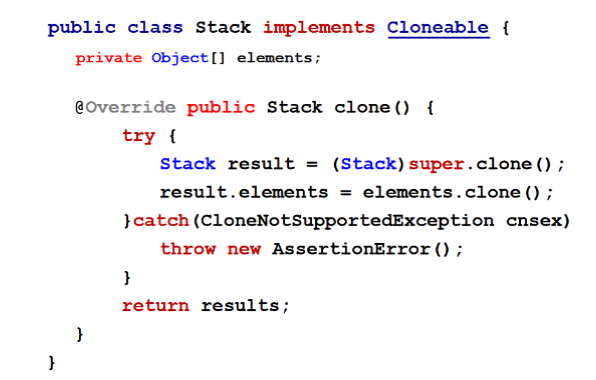
\includegraphics[scale=0.8]{images/deepCopyClone}
\caption{Deep copy Clone()\label{fig:UC3}}
\end{figure}
\begin{enumerate}
\item chiamare il metodo clone della superclasse;
\item castare il risultato al tipo stesso della classe;
\item si fa una copia profonda dei campiche hanno delle reference mutabili. Notare che su elements è stato chiamato clone()perché è il metodo che fa una copia profonda di un array di Objectma volendo si sarebbe potuto fare manualmente un for e fare deep copy del contenuto dell’array.;
\item i ritorna il risultato.
\end{enumerate}
La \textit{clone()} comunque potrebbe essere un problema se un campo è final, in generale è meglio avere un metodo di cloning separato e non implementare Cloneable.Ad esempio, si può usare un costruttore di copia oppure un factory method, ovvero un metodo che costruisce per me l’oggetto. Esempio di factory:
\begin{lstlisting}
public static Stack factoryNew(Stack source) {
Stack dest = new Stack(...);
	//faccio copie deep o altro prendendo i dati da source 
	return dest;
}
\end{lstlisting}
L’idea del factory è: creo un metodo da usare tipo Stack copia = Stack.factoryNew(...)che ritorna un oggetto di tipo Stack che è una copia esatta dell’oggetto che passoin input.